\chapter{Evaluation}
\label{chap:evaluation}

Dieses Kapitel widmet sich der Auswertung der Ergebnisse anhand verschiedener Metriken. Eingebettet in der Transformationssoftware befindet sich ein Präprozessor, der die aufgenommen Daten vor der Transformation manipulieren kann. Auf diese Weise werden mehrere Trainingsdatensätze erstellt, die in der Evaluation daraufhin analysiert werden, wie genau ein Klassifikator nach dem Training mit ihnen Vorhersagen treffen kann.

Die folgenden Datensätze werden generiert:

\begin{enumerate}
\item \textit{Combined}: Alle Daten werden ohne Veränderungen mit in die Transformation einbezogen.
\item \textit{NoisyBandTimestamps}: Die Zeitstempel der Readings des Bands werden mit gaussschem Rauschen versehen
\item \textit{Band combined}: Alle Daten des Smartphones werden vor der Transformation verworfen, sodass nur noch die Daten des Band verbleiben..
\item \textit{Band accel}: Nur die Daten des Beschleunigungssensors des Microsoft Band 2 werden mit in die Transformation einbezogen.
\item \textit{Band gyro}: Nur die Daten des Gyroskops des Microsoft Band 2 werden mit in die Transformation einbezogen.
\item \textit{Phone comb.}: Alle Daten des Microsoft Band 2 werden vor der Transformation verworfen, sodass nur noch die Daten des Smartphones verbleiben.
\item \textit{Phone accel}: Nur die Daten des Beschleunigungssensors des Smartphones werden mit in die Transformation einbezogen.
\item \textit{Phone gyro}: Nur die Daten des Gyroskops des Smartphones werden mit in die Transformation einbezogen.
\item \textit{SamplingRate1Hz}: Es werden Readings verworfen, als hätten Band und Smartphone jeweils nur Readings bei einer Rate von 1 Hz geliefert.
\item \textit{SamplingRate5Hz}: Es werden Readings verworfen, als hätten Band und Smartphone jeweils nur Readings bei einer Rate von 5 Hz geliefert.
\end{enumerate}

\section{Effektivität der Datenkombination}
Dieser Abschnitt widmet sich der Frage, wie effektiv die Kombination der Daten von Band und Smartphone hinsichtlich der Vorhersagegenauigkeit gegenüber einer einzigen Datenquelle ist. Weiss et al.\cite{Weiss2016} werten in ihrem Papier die Genauigkeit von Modellen aus, die entweder auf Daten des Beschleunigungssensors eines Smartphones, des Beschleunigungssensors einer Smartwatch oder des Gyroskops einer Smartwatch zurückgreifen. Eine Kombination der Daten schlagen die Autoren vor, führen diese allerdings nicht durch.

Tabelle~\ref{tab:accuracy-personal} zeigt die Genauigkeit der persönlichen Modelle und Tabelle~\ref{tab:accuracy-impersonal} die der unpersönlichen Modelle. Ein persönliches Modell basiert auf Daten des jeweiligen Benutzers, während ein unpersönliches Modell noch keine Daten des Nutzers gesehen hat, für den eine Vorhersage getroffen werden soll. Die \textit{Genauigkeit} ist definiert als der Anteil der korrekt klassifizierten Instanzen, die dem Modell zum Test vorgelegt wurden.

Die erste Spalte der in diesem Abschnitt referenzierten Tabellen gibt den Algorithmus an, der zur Klassifikation verwendet wurde. Eine Erläuterung der Algorithmen ist in Abschnitt~\ref{section:ml-algos}
zu finden. Fettgedruckt ist immer der jeweils höchste Wert einer Spalte.

\subsection{Persönliche Modelle}

Die Evaluierung der persönlichen Modelle erfolgt wie folgt: Für jeden Benutzer $b$ wird eine 10-fache Kreuzvalidierung durchgeführt, wobei die Trainingsdaten nur Daten von $b$ beinhalten. Anschließend wird der Durchschnitt der einzelnen Genauigkeiten über alle Benutzer gebildet, um einen globalen Genauigkeitswert zu erhalten. Um dieses Testverfahren zu ermöglichen, wurde die Weka-Software leicht angepasst: Die Methode zur Kreuzvalidierung wurde um einen Parameter $\texttt{foldSelector}: \texttt{Instanzen} \to \mathbb{N}$ erweitert, der für eine Instanz aus dem Datensatz zurückgibt, in welcher Iteration der Kreuzvalidierung diese aus dem Trainingsdatensatz ausgeschlossen und stattdessen im Testdatensatz verwendet wird.

Nutzt man nur je ein Gyroskop, ist die Qualität der persönlichen Modelle am schlechtesten. Im Gegensatz dazu haben bereits Modelle, die lediglich Daten von einem der Beschleunigungssensoren verwenden, eine gute Aussagekraft. Weiss et al.\cite{Weiss2016} stellten in ihrem Experiment fest, dass die Genauigkeit des \textit{Phone accel}-Modells $17.8 \%$ über dem \textit{Watch accel / Band accel}-Modell lag. Im eigenen Experiment ist der Unterschied trotz gleichem Experimentaufbau mit $1.6 \%$ weit geringer. Eine denkbare Erklärung wäre, dass die Probanden von Weiss et al. über verschiedene Aktivitäten hinweg mehr Variation bei ihrer Bewegung des Unterkörpers eingebracht haben könnten.

Vergleicht man \textit{Band accel} als die beste Datenquelle mit den Kombinationsmöglichkeiten, so lässt sich feststellen, dass die Hinzunahme der anderen Sensoren des Band eine Genauigkeit von $97.1 \%$ erzielt, wohingegen die Kombination der beiden Smartphone-Sensoren lediglich eine Verbesserung von $0.7 \%$ gegenüber \textit{Phone accel} und gegenüber \textit{Band accel} sogar eine Verschlechterung erwirkt. 

Hebt man jedoch diese künstlichen Einschränkungen auf, so wird eine Genauigkeit von $99.4 \%$ erreicht, sodass Benutzer nach dreiminütiger Aufnahme einer Aktivität davon ausgehen könnten, dass diese in Zukunft bis auf wenige Ausreißer automatisch erkannt wird. Insgesamt konnte gegenüber \textit{Phone Accel} damit eine Verbesserung um $9.4 \%$ erreicht werden. Gegenüber dem besten Ergebnis eines einzelnen Sensors (\textit{Band accel}) mit $91.6 \%$ liefert die Kombination aller Daten eine Verbesserung um $7.8 \%$.

\subsubsection{Vergleich mit Weiss et al.}
Da diese Bachelorarbeit auf der Arbeit von Weiss et al. \cite{Weiss2016} aufbaut, ist ein Vergleich der Ergebnisse sinnvoll. Abbildung~\ref{fig:accuracy-personal-vs-weiss} zeigt die Genauigkeiten der besten Modelle in Abhängigkeit von den Datenquellen. Sowohl die Quellen \textit{Watch accel} als auch \textit{Watch gyro} liefern sehr ähnliche Ergebnisse wie bei Weiss et al., nur das \textit{Phone accel}-Modell in dieser Arbeit liefert im direkten Vergleich eine deutlich bessere Genauigkeit. Eine mögliche Erklärung wäre die im Vergleich mit Weiss et al. 10-fach höhere Sampling-Rate des Sensoren des Smartphones gewesen, jedoch lieferte ein Test mit einem RF-Modell und auf 20 Hz beschränkten Smartphone-Daten immerhin noch eine Genauigkeit von $88.2 \%$. Da dies dennoch $12.7 \%$ über dem \textit{Phone Accel}-Modell von Weiss et al. liegt, lässt sich diese Erklärung ausschließen. Eine weitere Erklärungsmöglichkeit wäre, dass die Genauigkeit des Sensors im OnePlus 3 über der des Sensors im Samsung Galaxy S4 liegt, das von Weiss et al. zur Aufnahme genutzt wird, jedoch kann diese Hypothese mangels eines solchen Gerätes nicht verifiziert werden. Die Methodik zur Reduktion der Sampling-Rate wird in Abschnitt~\ref{sec:lower-sampling-rate} erklärt, der sich weiteren solchen Analysen widmet.

Erwartungsgemäß ist die Genauigkeit mit den vollständig kombinierten Datenquellen arbeitsübergreifend am höchsten, jedoch ist dies sogar der Fall, wenn man die Daten des Smartphones entfernt. Nutzt man hingegen nur die Daten des Smartphones, ist die Genauigkeit vergleichbar mit den beiden \textit{Watch accel}-Ergebnisse.


\begin{figure}
\centering
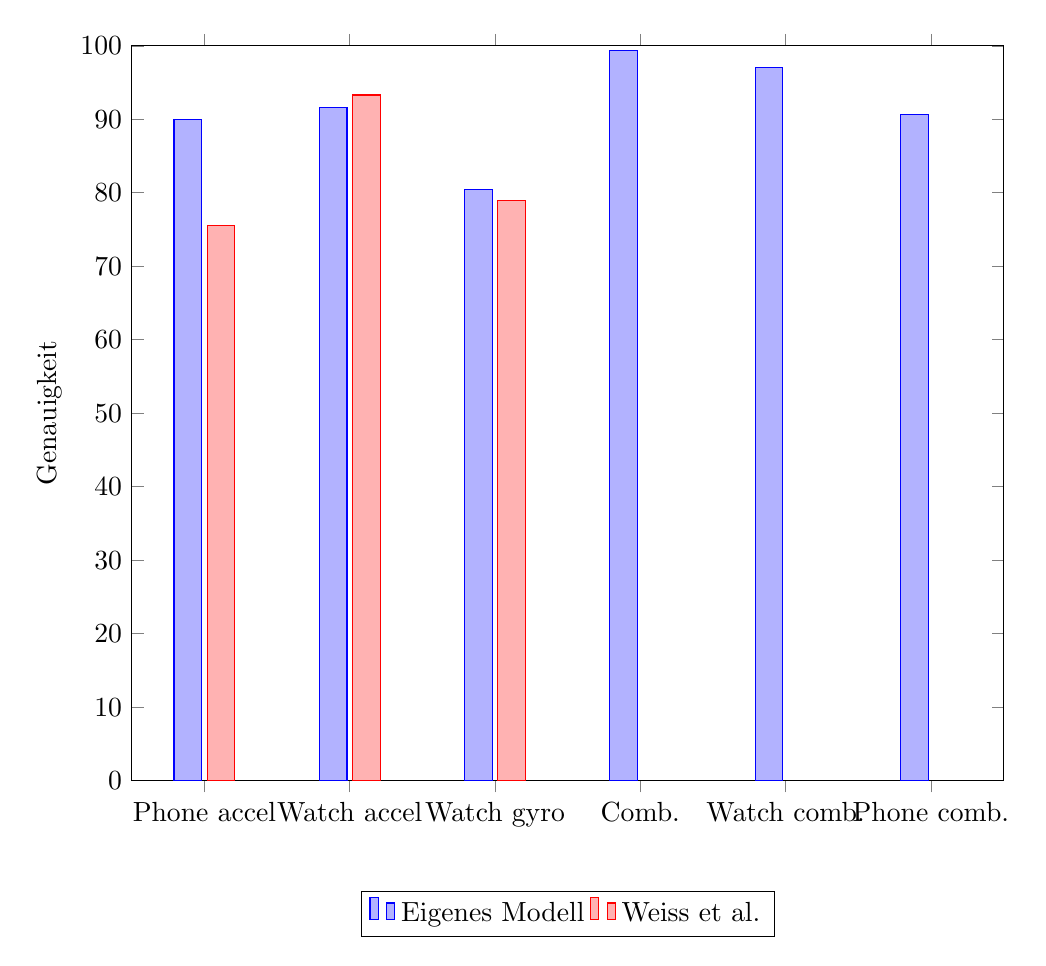
\begin{tikzpicture}
\begin{axis}[
width=360pt,
xtick=data,
ymin=0,
ymax=100,
ylabel=Genauigkeit,
symbolic x coords={Phone accel,Watch accel,Watch gyro,Comb.,Watch comb.,Phone comb.},
legend style={at={(0.5,-0.15)},
	anchor=north,legend columns=-1},
ybar,
]
\addplot 
coordinates {(Phone accel,90) (Watch accel,91.6) (Watch gyro,80.5) (Comb.,99.4) (Watch comb.,97.1) (Phone comb.,90.7)};

\addplot 
coordinates {(Phone accel,75.5) (Watch accel,93.3) (Watch gyro,79)};

\legend{Eigenes Modell,Weiss et al.}
\end{axis}
\end{tikzpicture}
\caption[Vergleich der Genauigkeiten der persönlichen Modelle mit Weiss et al.\cite{Weiss2016}]{Vergleich der Genauigkeiten der persönlichen Modelle mit Weiss et al.\cite{Weiss2016}. Die \textit{Watch} ist in dieser Arbeit das Band.}
\label{fig:accuracy-personal-vs-weiss}
\end{figure}

\subsection{Unpersönliche Modelle}
\label{subsec:eval-impersonal-models}
Für die Evaluierung der unpersönlichen Modelle wird eine Kreuzvalidierung über die Nutzer durchgeführt, das heißt der Datensatz $D$ wird für alle Benutzer $b$ aufgeteilt in $D = \text{Train} \uplus \text{Test}$ mit $\text{Train} = \{\text{Intervall ist nicht von } b\}, \text{Test} = D \backslash \text{Train}$.

Das schlechteste Ergebnis wird mit $35.1 \%$ bei den unpersönlichen Modellen erzielt, wenn nur das Gyroskop des Smartphones verwendet wird. Nur wenig besser sind die Modelle, die nur den Beschleunigungssensor des Smartphones ($39.2 \%$) oder beide Sensoren des Smartphones ($41.3 \%$) nutzen. Für den praktischen Gebrauch sind diese Modelle aufgrund ihrer Ungenauigkeit untauglich. Schon rund $20 \%$ besser sind die Modelle, die nur das Gyroskop des Bands nutzen, wobei der Wechsel zum Beschleunigungssensor eine weitere Verbesserung um fast $14 \%$ ermöglicht. Offenbar erklären die Daten des Beschleunigungssensors einen Großteil der Daten, die auch durch das Gyroskop und die anderen Sensoren des Band erklärt werden, sodass eine Kombination aller Band-Sensoren lediglich ein Verbesserung um rund $1 \%$ ermöglicht. Selbiges gilt auch für die Hinzunahme der Daten des Smartphones: Es wird eine Verbesserung um $2 \%$ erzielt, was darauf schließen lässt, dass die Armbewegungen unter den Probanden ähnlich sind, die Bewegungen auf Hüfthöhe hingegen weniger. Gegenüber dem besten Ergebnis eines einzelnen Sensors (\textit{Band accel}) mit $75.2 \%$ liefert die Kombination aller Daten eine Verbesserung um $3.3 \%$.

\subsubsection{Vergleich mit Weiss et al.}
Im Gegensatz zu den persönlichen Modellen unterscheiden sich die unpersönlichen Modelle allesamt um weniger als 5 Prozent von denen von Weiss et al. Auffällig ist, dass die Kombination der Sensoren des Smartphones auch im Vergleich mit Weiss et al. keine nennenswerte Verbesserung liefert, dafür jedoch das Einbeziehen der Sensoren des Bands für signifikant bessere Ergebnisse sorgt. Die vollständige Kombination liefert beispielsweise eine um $8.3 \%$ höhere Genauigkeit als das mit $70.3 \%$ bei Weiss et al. im Vergleich mit dem eigenen Modell leicht bessere \textit{Watch accel}-Modell.

\begin{figure}
	\centering
	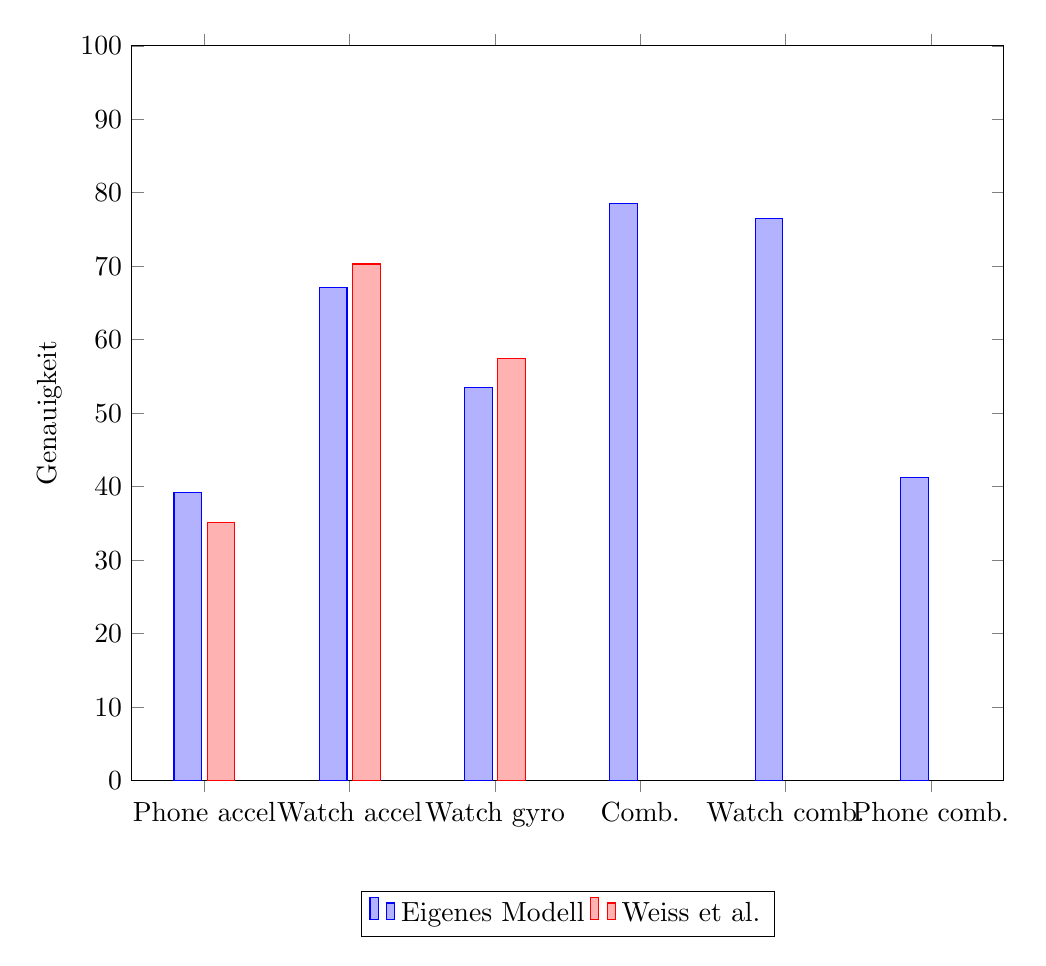
\begin{tikzpicture}
	\begin{axis}[
	width=360pt,
	xtick=data,
	ymin=0,
	ymax=100,
	ylabel=Genauigkeit,
	symbolic x coords={Phone accel,Watch accel,Watch gyro,Comb.,Watch comb.,Phone comb.},
	legend style={at={(0.5,-0.15)},
		anchor=north,legend columns=-1},
	ybar,
	]
	\addplot 
	coordinates {(Phone accel,39.2) (Watch accel,67.1) (Watch gyro,53.5) (Comb.,78.5) (Watch comb.,76.5) (Phone comb.,41.3)};
	
	\addplot 
	coordinates {(Phone accel,35.1) (Watch accel,70.3) (Watch gyro,57.5)};
	
	\legend{Eigenes Modell,Weiss et al.}
	\end{axis}
	\end{tikzpicture}
	\caption[Vergleich der Genauigkeiten der unpersönlichen Modelle mit Weiss et al.\cite{Weiss2016}]{Vergleich der Genauigkeiten der unpersönlichen Modelle mit Weiss et al.\cite{Weiss2016}. Die \textit{Watch} ist in dieser Arbeit das Band.}
	\label{fig:accuracy-impersonal-vs-weiss}
\end{figure}

\begin{table}
\centering
\begin{tabular}{|c|c|c|c|c|c|c|c|}
	\hline 
	\textbf{Algo.} & \textbf{Phone accel} & \textbf{Phone gyro} & \textbf{Band accel} & \textbf{Band gyro} & \textbf{Comb.} & \textbf{Band comb.} & \textbf{Phone comb.} \\ 
	\hline 
	RF & 88.7 & \textbf{68.2} & \textbf{91.6} & \textbf{80.5} & \textbf{99.4} & \textbf{97.1} & \textbf{90.7} \\ 
	J48 & \textbf{90.0} & 64.3 & 86.5 & 72.7 & 92.8 & 90.1 & 89.7 \\ 
	IB3 & 62.2 & 44.8 & 77.0 & 59.4 & 82.3 & 76.9 & 60.1 \\ 
	NB & 87.6 & 60.4 & 90.9 & 78.8 & 96.2 & 92.2 & 85.5 \\ 
	MLP & 78.9 & 51.5 & 88.9 & 67.8 & 94.8 & 90.7 & 75.1 \\ 
	\hline 
	$\varnothing$ & 81.5 & 57.8 & 87.0 & 71.8 & 93.1 & 89.4 & 80.2 \\ 
	\hline 
\end{tabular}
\caption{Genauigkeit der persönlichen Modelle in Prozent}
\label{tab:accuracy-personal}
\end{table}

\begin{table}
\centering
\begin{tabular}{|c|c|c|c|c|c|c|c|}
	\hline 
	\textbf{Algo.} & \textbf{Phone accel} & \textbf{Phone gyro} & \textbf{Band accel} & \textbf{Band gyro} & \textbf{Comb.} & \textbf{Band comb.} & \textbf{Phone comb.} \\ 
	\hline 
	RF & \textbf{39.2} & \textbf{35.1} & \textbf{75.2} & \textbf{61.7} & \textbf{78.5} & \textbf{76.5} & \textbf{41.3} \\ 
	J48 & 32.9 & 29.1 & 61.6 & 49.2 & 59.7 & 61.3 & 32.6 \\ 
	IB3 & 24.3 & 22.6 & 60.9 & 45.0 & 52.9 & 58.0 & 26.0 \\ 
	NB & 31.8 & 30.0 & 67.3 & 56.9 & 60.9 & 62.3 & 35.0 \\ 
	MLP & 28.8 & 29.3 & 70.3 & 53.5 & 54.9 & 74.3 & 31.5 \\ 
	\hline 
	$\varnothing$ & 81.5 & 29.2 & 67.1 & 53.3 & 61.4 & 66.5 & 33.3 \\ 
	\hline 
\end{tabular} 
\caption{Genauigkeit der unpersönlichen Modelle in Prozent}
\label{tab:accuracy-impersonal}
\end{table}

\section{Genauigkeit bei ungenauen Zeitstempeln}
Die Problemstellung, Daten mehrerer Quellen miteinander zu kombinieren, wirft die Frage auf, inwiefern die Synchronisierung der Daten einen Einfluss auf die Genauigkeit der resultierenden Modelle besitzt. Smartphone und Band besitzen je eine eigene Uhr, sodass die Datenquellen zum selben Zeitpunkt $t$ \textit{Readings} mit Zeitstempeln $t + \epsilon_\text{Smartphone}$, bzw. $t + \epsilon_\text{Band}$ mit $|\epsilon_\text{Smartphone} - \epsilon_\text{Band}| > 0$ liefern könnten. Wird die Differenz zu groß, schadet die Kombination der Quellen möglicherweise mehr als sie nützt.

Ein erster Ansatz, um dieses Problem zu bekämpfen, war daher zunächst, die beiden Uhren via Bluetooth und einem Verfahren wie das \textit{Network Time Protocol (NTP)} \cite{Mills} zu synchronisieren. Leider ermöglicht das Microsoft Band SDK nicht die Ausführung beliebigen Codes auf dem Band, sondern nur das Abonnieren von Sensordaten-Events, weshalb kein direkter Zugriff auf die Uhr des Gerätes möglich ist. Die Events sind zwar mit Zeitstempeln versehen, jedoch kann die Übertragungszeit nicht ermittelt werden. Eine manuelle Synchronisierung der Uhren ist daher nicht möglich.

Um zu prüfen, inwiefern die Modelle durch eine mögliche, nicht detektierbare Differenz der Uhren beeinträchtigt werden, generiert die Transformationssoftware zusätzlich zum normalen vollständigen Datensatz auch einen, in dem die Zeitstempel des Bands additiv mit gausschem Rauschen versehen wurden. Die Parameter des gausschen Rauschens wurden auf einen Mittelwert von $0$ und eine Standardabweichung von $500 \text{ms}$ festgelegt. Die Ergebnisse der Auswertung werden in Tabelle~\ref{tab:accuracy-noisy_timestamps} aufgeführt. Betrachtet man die jeweils besten Modelle, so lässt sich sowohl bei den persönlichen, als auch bei den unpersönlichen Modellen eine Verschlechterung um lediglich $0.2 \%$ feststellen. Auch die anderen Modelle sind im Durchschnitt mit Verschlechterungen um $0.3 \%$, bzw. $0.5 \%$ hinreichend resistent gegen das Rauschen.

Um zu prüfen, ob eine Standardabweichung von $500 \text{ms}$ sinnvoll ist, wurde über drei Tage hinweg um jeweils 10, 15 und 18 Uhr geprüft, mit welchem zeitlichen Abstand das Umspringen von der vollen Stunde auf die nächste Minute erfolgte. Eine Verzögerung war in keinem der Fälle mit dem Auge beobachtbar, weshalb davon auszugehen ist, dass die Uhren aufgrund der bereits bestehenden Synchronisierung durch die vom Hersteller gelieferte Band-App für Android in der Regel weniger als $500 \text{ms}$ voneinander abweichen. Dies führt zu der Annahme, dass die Genauigkeit der Zeitstempel im Rahmen dieser Arbeit keinen negativen Einfluss auf die Ergebnisse hat und somit nicht weiter betrachtet werden muss.

\begin{table}
\centering
\begin{tabular}{|c|c|c||c|c|}
	\hline 
	\textbf{Algo.} & \textbf{Comb. (Pers.)} & \textbf{Verrauscht (Pers.)} &\textbf{Comb. (Unpers.)} & \textbf{Verrauscht (Unpers.)} \\ 
	\hline 
	RF & \textbf{99.4} & \textbf{99.2} & \textbf{78.5} & \textbf{78.3} \\ 
	J48 & 92.8 & 93.5 & 59.7 & 57.3 \\ 
	IB3 & 82.3 & 81.5 & 52.9 & 52.9 \\ 
	NB & 96.2 & 95.7 & 60.9 & 60.5 \\ 
	MLP & 94.8 & 94.2 & 54.9 & 55.4 \\ 
	\hline 
	$\varnothing$ & 93.1 & 92.8 & 61.4 & 60.9 \\ 
	\hline
\end{tabular} 
\caption{Genauigkeit der Modelle mit verrauschten Band-Zeitstempeln in Prozent}
\label{tab:accuracy-noisy_timestamps}
\end{table}

\section{Genauigkeit bei einer niedrigen Sampling-Rate}
\label{sec:lower-sampling-rate}
Da beide verwendete Geräte primär akkubetrieben sind, muss bei einer marktreifen Umsetzung einer Aufnahmesoftware auch bedacht werden, dass das Sammeln der Daten hinsichtlich der Energieressourcen nicht kostenlos ist. Eine Rolle beim Energieverbrauch spielt auch die Sampling-Rate (Abtastrate): Ist sie hoch eingestellt, können die entsprechenden Sensoren nicht in einen Energiesparmodus wechseln und außerdem müssen von der anfordernden Anwendung mehr Daten verarbeitet werden, wodurch wiederum Anforderungen an den Prozessor gestellt werden \cite{Krause2005}. Beim Band kommt hinzu, dass eine höhere Bluetooth-Datenrate in Kauf genommen werden muss, die insbesondere auf den bauartbedingt kleinen Akku des Fitness-Trackers einen negativen Einfluss hat. Aus diesem Grund ist es untersuchenswert, inwiefern die Sampling-Rate einen Einfluss auf die Genauigkeit der Modelle besitzt, um möglicherweise Energie sparen zu können.

Die Sampling-Raten, mit denen die Aufnahmesoftware Daten aufgezeichnet hat, befinden sich in Tabelle~\ref{tab:sampling-rates}. Um Sampling-Raten miteinander zu vergleichen, wurden dieselben Rohdaten verwendet wie im normalen, vollständigen Modell. Um eine Sampling-Rate von $k$ Hz zu simulieren, wurden nach einem behaltenen Reading $(t_0\,\text{secs}, \text{sensor}, \text{source}, ...)$ alle weiteren Readings $(t\,\text{secs}, \text{sensor}, \text{source}, ...)$ mit $t \in [t_0, t_0 + 1/k]$ gelöscht.

Nun werden die besten Modelle miteinander verglichen. Zur Erinnerung: \textit{Comb. (Pers.)} erzielte eine Genauigkeit von $99.4 \%$ und \textit{Comb. (Unpers.)} eine Genauigkeit von $78.5 \%$. Reduziert man die Sampling-Rate des persönlichen Modells auf 5 Hz, so reduziert sich die Genauigkeit um $0.8 \%$. Eine dramatischere Verschlechterung wird durch die Reduzierung auf 1 Hz verursacht, durch die sich die Genauigkeit um $4.1 \%$ verschlechtert. Noch stärker beeinträchtigt werden durch die Reduzierung der Sampling-Rate die unpersönlichen Modelle. Beschränkt man diese auf 5 Hz, so ergibt sich gegenüber \textit{Comb. (Unpers.)} eine Verschlechterung um $8.4 \%$. Bei einer Beschränkung auf 1 Hz beträgt die Verschlechterung sogar $16.4 \%$, sodass zu einer Reduzierung der Sampling-Rate nur bei den ohnehin bereits genauen persönlichen Modellen zu raten ist.

\begin{table}
\centering
\begin{tabular}{|c|c|c|}
	\hline 
	\textbf{Gerät} & \textbf{Sensor} & \textbf{Durchsch. Sampling-Rate} \\ 
	\hline 
	Smartphone & Accelerometer & 200 Hz \\ 
	\hline 
	Smartphone & Gyroskop & 200 Hz \\ 
	\hline 
	Fitness-Tracker & Accelerometer & 8 Hz \\ 
	\hline 
	Fitness-Tracker & Gyroskop & 8 Hz \\ 
	\hline 
	Fitness-Tracker & Laufgeschwindigkeit & 1 Hz \\ 
	\hline 
	Fitness-Tracker & Hautwiderstand & 5 Hz \\ 
	\hline 
\end{tabular}
\caption{Sampling-Raten der Sensoren}
\label{tab:sampling-rates}
\end{table}

\begin{table}
\centering
\begin{tabular}{|c|c|c||c|c|}
	\hline 
	\textbf{Algo.} & \textbf{5 Hz (Pers.)} & \textbf{1 Hz (Pers.)} &\textbf{5 Hz (Unpers.)} & \textbf{1 Hz (Unpers.)} \\ 
	\hline 
	RF & \textbf{98.6} & \textbf{95.3} & \textbf{70.1} & \textbf{62.1} \\ 
	J48 & 93.8 & 87.8 & 53.4 & 48.7 \\ 
	IB3 & 71.0 & 14.6 & 43.5 & 7.8 \\ 
	NB & 91.6 & 75.5 & 53.3 & 44.2 \\ 
	MLP & 90.0 & 78.9 & 63.6 & 51.2 \\ 
	\hline 
	$\varnothing$ & 89.0 & 70.4 & 56.8 & 42.8 \\ 
	\hline
\end{tabular} 
\caption{Genauigkeit der Modelle mit reduzierter Sampling-Rate in Prozent}
\label{tab:accuracy-sampling_rate}
\end{table}

\section{Genauigkeit bei Überlappung der Intervalle}
\begin{figure}[htb]
\centering
\includegraphics[clip=true, trim=5mm 5mm 5mm 5mm]{img/interval_overlap}
\caption{Intervallüberlappung}
\label{fig:interval-overlap}
\end{figure}

Bao et al. nutzten 2004 auf der Basis bereits bestehender Werke für die Transformation eine Intervallüberlappung von $50 \%$ \cite{Bao2004}. Weiss et al. probierten dies laut ihrem Paper nicht aus \cite{Weiss2016}. Um zu prüfen, ob dies eine weitere Verbesserung der Genauigkeiten erzielen könnte, wurden für die Intervalle $(t_0, t_0 + 10), ((t_0 + 10) - 10 * 0.5, (t_0 + 10) - 10 * 0.5 + 10), ...$ Features generiert und wie zuvor evaluiert. Eine Illustration der Überlappung befindet sich in Abbildung~\ref{fig:interval-overlap}.

Anders als erhofft verschlechterten sich die persönlichen RF-Modelle wie in Tabelle~\ref{tab:accuracy-overlap} ersichtlich durch die Überlappung um $0.2 \%$, während sich die unpersönlichen Modelle sogar um $5.1 \%$ verschlechterten.

\begin{table}
\centering
\begin{tabular}{|c|c|c||c|c|}
	\hline 
	\textbf{Algo.} & \textbf{Comb. (Pers.)} & \textbf{Überlappung (Pers.)} &\textbf{Comb. (Unpers.)} & \textbf{Überlappung (Unpers.)} \\ 
	\hline 
	RF & \textbf{99.4} & \textbf{99.2} & \textbf{78.5} & \textbf{73.4} \\ 
	J48 & 92.8 & 96.3 & 59.7 & 57.5 \\ 
	IB3 & 82.3 & 81.8 & 52.9 & 50.7 \\ 
	NB & 96.2 & 95.8 & 60.9 & 59.7 \\ 
	MLP & 94.8 & 95.0 & 54.9 & 59.4 \\ 
	\hline 
	$\varnothing$ & 93.1 & 93.6 & 61.4 & 60.9 \\ 
	\hline
\end{tabular} 
\caption{Genauigkeit der Modelle mit Intervallüberlappung in Prozent}
\label{tab:accuracy-overlap}
\end{table}

\section{Genauigkeit bei Verschmelzung der Ess- und Trinkaktivitäten}
\begin{table}
\centering
\begin{tabular}{|c|c|c|}
	\hline 
	\textbf{Algo.} & \textbf{Comb. (Unpers.), verschmolzen} & \textbf{Comb. (Unpers.), nicht verschmolzen} \\ 
	\hline 
	RF & \textbf{87.1} &  \textbf{78.5} \\ 
	J48 & 73.7 &  59.7 \\ 
	IB3 & 63.9 &  52.9  \\ 
	NB & 72.4 & 60.9  \\ 
	MLP & 77.6  & 54.9 \\ 
	\hline 
	$\varnothing$ & 74.9 & 61.4  \\ 
	\hline
\end{tabular} 
\caption{Genauigkeit der Modelle bei Verschmelzung der Ess- und Trinkaktivitäten in Prozent}
\label{tab:accuracy-merge-eating}
\end{table}
\begin{sidewaystable}
\centering
\begin{tabular}{|c|c|c|c|c|c|c|c|c|c|c|c|c|c|c|c|c|c||l|}
\hline 
\textbf{a} &  \textbf{b} & \textbf{c} & \textbf{d} & \textbf{e} & \textbf{f} & \textbf{g} & \textbf{h} & \textbf{i} & \textbf{j} & \textbf{k} & \textbf{l} & \textbf{m} & \textbf{n} & \textbf{o} & \textbf{p} & \textbf{q} & \textbf{r} & \textbf{$<$ Output für $\vee$} \\
\hline 
\hline 
149 & 0 & 0 & 0 & 0 & 0 & 2 & 0 & 0 & 8 & 0 & 0 & 0 & 2 & 0 & 0 & 0 & 0 & \textbf{a = Brushing Teeth} \\
\hline 
0 & 153 & 0 & 7 & 0 & 0 & 0 & 0 & 0 & 0 & 0 & 0 & 0 & 1 & 0 & 0 & 0 & 0 & \textbf{b = Clapping} \\
\hline 
0 & 0 & 126 & 0 & 0 & 0 & 0 & 0 & 0 & 0 & 0 & 1 &17 & 0 & 0 & 0 & 0 & 26 & \textbf{c = Climbing Stairs} \\
\hline 
0 & 11 & 0 & 147 & 0 & 0 & 0 & 0 & 0 & 1 & 0 & 0 & 0 & 5 & 0 & 0 & 0 & 0 & \textbf{d = Basketball} \\
\hline 
0 & 0 & 0 & 0 & \cellcolor{lightgray} 133 & \cellcolor{lightgray} 6 & \cellcolor{lightgray} 0 & \cellcolor{lightgray} 9 & \cellcolor{lightgray}  0 & 0 & 0 & 0 & 0 & 0 & 12 & 0 & 3 & 0 & \textbf{e = Drinking} \\
\hline 
1 & 0 & 0 & 0 & \cellcolor{lightgray} 5 & \cellcolor{lightgray} 135 & \cellcolor{lightgray} 3 & \cellcolor{lightgray} 15 & \cellcolor{lightgray} 4 & 0 & 0 & 0 & 0 & 0 & 0 & 0 & 1 & 0 & \textbf{f = Eating Chips} \\
\hline 
3 & 0 & 0 & 0 & \cellcolor{lightgray} 0 & \cellcolor{lightgray} \cellcolor{lightgray} 11 & \cellcolor{lightgray} 106 & \cellcolor{lightgray} 3 & \cellcolor{lightgray} 24 & 0 & 3 & 0 & 0 & 0 & 2 & 0 & 9 & 0 & \textbf{g = Eating Pasta} \\
\hline 
3 & 0 & 0 & 0 & \cellcolor{lightgray} 14 & \cellcolor{lightgray} 26 & \cellcolor{lightgray} 15 & \cellcolor{lightgray} 75 & \cellcolor{lightgray} 27 & 0 & 6 & 0 & 0 & 0 & 7 & 1 & 3 & 0 & \textbf{h = Eating Sandwich} \\
\hline 
7 & 0 & 0 & 0 & \cellcolor{lightgray} 0 & \cellcolor{lightgray} 13 & \cellcolor{lightgray} 39 & \cellcolor{lightgray} 44 & \cellcolor{lightgray} 84 & 0 & 0 & 0 & 0 & 0 & 3 & 0 & 2 & 0 & \textbf{i = Eating Soup} \\
\hline 
6 & 0 & 0 & 0 & 0 & 0 & 0 & 0 & 0 & 148 & 0 & 0 & 3 & 2 & 0 & 0 & 0 & 0 & \textbf{j = Folding Clothes} \\
\hline 
0 & 0 & 0 & 0 & 0 & 5 & 7 & 6 & 2 & 0 & 139 & 0 & 0 & 0 & 0 & 0 & 4 & 0 & \textbf{k = Handwriting} \\
\hline 
0 & 0 & 2 & 0 & 0 & 0 & 0 & 0 & 0 & 0 & 0 & 166 & 0 & 0 & 0 & 0 & 0 & 0 & \textbf{l = Jogging} \\
\hline 
0 & 0 &13 & 0 & 0 & 0 & 0 & 0 & 0 & 0 & 0 & 1 & 150 & 0 & 0 & 0 & 0 & 2 & \textbf{m = Soccer Ball} \\
\hline 
0 & 0 & 0 & 7 & 0 & 0 & 0 & 0 & 0 & 0 & 0 & 0 & 3 & 145 & 0 & 0 & 0 & 0 & \textbf{n = Playing Catch} \\
\hline 
4 & 0 & 0 & 0 & 1 & 2 & 2 & 1 & 1 & 0 & 4 & 0 & 0 & 0 & 136 & 8 & 5 & 0 & \textbf{o = Sitting} \\
\hline 
1 & 0 & 0 & 0 & 0 & 0 & 0 & 1 & 0 & 0 & 0 & 0 & 1 & 0 &15 & 142 & 0 & 0 & \textbf{p = Standing} \\
\hline 
2 & 0 & 0 & 0 & 1 & 1 & 4 & 1 & 0 & 0 & 27 & 0 & 0 & 0 & 0 & 0 & 125 & 0 & \textbf{q = Typing} \\
\hline 
0 & 0 &66 & 0 & 0 & 0 & 0 & 0 & 0 & 0 & 0 & 0 & 19 & 0 & 0 & 0 & 0 & 84 & \textbf{r = Walking} \\
\hline 
\end{tabular}
\caption{Konfusionsmatrix der unpersönlichen RF-Modelle}
\label{tab:confusion-impersonal-rf}
\end{sidewaystable}

Betrachtet man die Konfusionsmatrix der vollständigen unpersönlichen RF-basierten Modelle in Tabelle~\ref{tab:confusion-impersonal-rf}, so lässt sich feststellen, dass die Klassen, die sich mit Essen oder Trinken beschäftigen, nur ungenau erkannt werden und somit die Durchschnittsgenauigkeit entsprechend senken. Zudem liegt die fehlerhaft vorhergesagte Klasse in $298/324 \approx 92 \%$ der Fälle im Bereich des Essens und Trinkens. Zurückzuführen ist dies auf die Tatsache, dass sich diese Aktivitäten untereinander ähneln, da die zentralen Bewegungsmerkmale bei all diesen Klassen das Sitzen sowie das Führen der Hand zum Mund sind.

\begin{sidewaystable}
\centering
\begin{tabular}{|c|c|c|c|c|c|c|c|c|c|c|c|c|c||l|}
	\hline 
  \textbf{a} &   \textbf{b} &   \textbf{c} &   \textbf{d} &   \textbf{e} &   \textbf{f} &   \textbf{g} &   \textbf{h} &   \textbf{i} &   \textbf{j} &   \textbf{k} &   \textbf{l} &   \textbf{m}  &  \textbf{n} & \textbf{$<$ Output für $\vee$} \\
\hline 
\hline
143 &   0 &   0 &   0 &   5 &  12 &   0 &   0 &   0 &   1 &   0 &   0 &   0  &  0 &   \textbf{a = Brushing Teeth} \\
\hline 
0 & 155 &   0 &   5 &   0 &   0 &   0 &   0 &   0 &   1 &   0 &   0 &   0  &  0 &   \textbf{b = Clapping} \\
\hline 
0 &   0 & 126 &   0 &   0 &   0 &   0 &   1 &  13 &   0 &   0 &   0 &   0  & 30 &   \textbf{c = Climbing Stairs} \\
\hline 
0 &   5 &   0 & 136 &   0 &   5 &   0 &   0 &   0 &  18 &   0 &   0 &   0  &  0 &   \textbf{d = Basketball} \\
\hline 
2 &   0 &   0 &   0 & 830 &   0 &   2 &   0 &   0 &   0 &  16 &   0 &   7  &  0 &   \textbf{e = Eating} \\
\hline 
2 &   0 &   0 &   0 &   0 & 155 &   0 &   0 &   0 &   2 &   0 &   0 &   0  &  0 &   \textbf{f = Folding Clothes} \\
\hline 
0 &   0 &   0 &   0 &  30 &   0 & 124 &   0 &   0 &   0 &   0 &   0 &   9  &  0 &   \textbf{g = Handwriting} \\
\hline 
0 &   0 &   0 &   0 &   0 &   0 &   0 & 168 &   0 &   0 &   0 &   0 &   0  &  0 &   \textbf{h = Jogging} \\
\hline 
0 &   0 &   6 &   0 &   0 &   0 &   0 &   1 & 157 &   1 &   0 &   0 &   0  &  1 &   \textbf{i = Soccer Ball} \\
\hline 
0 &   0 &   0 &   7 &   0 &   2 &   0 &   1 &   2 & 143 &   0 &   0 &   0  &  0 &   \textbf{j = Playing Catch} \\
\hline 
1 &   0 &   0 &   0 &  23 &   0 &   2 &   0 &   0 &   0 & 130 &   8 &   0  &  0 &   \textbf{k = Sitting} \\
\hline 
0 &   0 &   0 &   0 &   5 &   0 &   0 &   0 &   0 &   0 &  17 & 138 &   0  &  0 &   \textbf{l = Standing} \\
\hline 
1 &   0 &   0 &   0 &  37 &   0 &  18 &   0 &   0 &   0 &   0 &   0 & 105  &  0 &   \textbf{m = Typing} \\
\hline 
0 &   0 &  60 &   0 &   0 &   0 &   0 &   0 &  26 &   0 &   0 &   0 &   0  & 83 &   \textbf{n = Walking} \\
	\hline 
\end{tabular}
\caption{Konfusionsmatrix der unpersönlichen, verschmolzenen RF-Modelle}
\label{tab:confusion-impersonal-rf-merged}
\end{sidewaystable}

Tabelle~\ref{tab:accuracy-merge-eating} zeigt, wie sich die Genauigkeit der unpersönlichen Modelle verändert, wenn man diese Aktivitäten zu einer einzigen Aktivität verschmilzt. Bei den RF-Modellen ist eine Verbesserung um $8.6 \%$ zu erkennen, wovon ein Teil auch darauf zurückzuführen sein könnte, dass es insgesamt weniger Klassen gibt und die Wahrscheinlichkeit einer Fehlklassifikation somit sinkt. Tabelle~\ref{tab:confusion-impersonal-rf-merged} zeigt die neue Konfusionsmatrix der RF-Modelle und es wird deutlich, dass aufgrund der verschmolzenen Aktivität \textit{Eating} die Fehlerrate stark gesunken ist.

Aus diesen Daten lässt sich schließen, dass bei der Verwendung von unpersönlichen Modellen darauf geachtet werden sollte, dass die zu erkennenden Aktivitäten nicht zu feingranular voneinander getrennt werden, da dies die Klassifikation stark erschweren kann.

\section{Genauigkeit in Abhängigkeit von der Teilnehmeranzahl}
Während die persönlichen Modelle lediglich auf die Bewegungsdaten einer einzelnen Person zurückgreifen, sind für die unpersönlichen Modelle Daten anderer Personen erforderlich. Daraus ergibt sich die Frage, wie die Genauigkeit der unpersönlichen Modelle von der Anzahl der Personen, auf denen dieses basiert, abhängig it. Um dies zu ermitteln, wurden aus dem aus 10 Personen bestehenden vollständigen Datensatz $D$ für $i \in \{2, ..., 10\}$ je $N_i := \min(10, \binom{10}{i})$ verschiedene, zufällig gezogene Datensätze $D_{i,j}$ mit $j \in \{1, ..., N_i\}$ generiert. Ein Datensatz $D_{i,j}$ enthält Daten von $i \geq 2$ verschiedenen Personen, um die Aufteilung in Train- und Testsets zu ermöglichen, da ein Testset für die unpersönlichen Modelle genau eine Person enthalten soll und die Mengen disjunkt sein müssen (vgl. Abschnitt~\ref{subsec:eval-impersonal-models}). Die Genauigkeit in Abhängigkeit von der Anzahl der Personen $i$ ist dann definiert durch $G(i) := \sum_{j=1}^{N_i} \frac{\text{Genauigkeit mit } D_{i,j}}{N_i}$. Die Berechnung der Genauigkeit mit Datensatz $D_{i,j}$ erfolgt nach Abschnitt~\ref{subsec:eval-impersonal-models}.
\todo{Visuelle Illustration des Ziehens von Datensätzen}
Abbildung~\ref{fig:accuracy-convergence} zeigt den Plot der Funktion $G$. Es ist zu erkennen, dass die Genauigkeit langsam konvergiert, wobei für $i > 10$ noch etwas höhere Genauigkeiten zu erwarten sind. Die Verifikation dieser Hypothese durch weitere Aufnahmen war im Rahmen der zeitlichen Beschränkungen einer Bachelorarbeit nicht möglich.

\begin{figure}
\centering
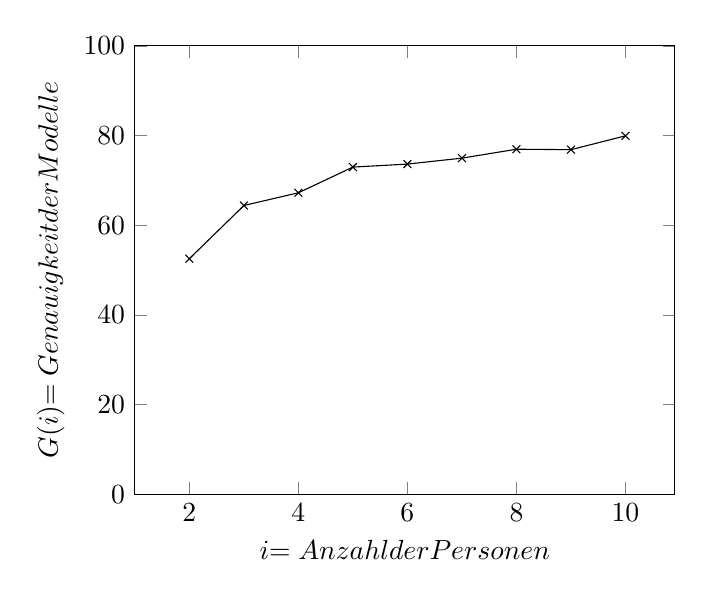
\begin{tikzpicture}
\begin{axis}[
ymin=0,
ymax=100,
xmin=1,
xlabel=$i \text{ = Anzahl der Personen}$,
ylabel=$G(i) \text{ = Genauigkeit der Modelle}$]
\addplot[color=black,mark=x] coordinates {
	(2, 52.52308602)
	(3, 64.3778887)
	(4, 67.2191227465409)
	(5, 72.94877937)
	(6, 73.61805308)
	(7, 74.9440529)
	(8, 76.93207282)
	(9, 76.83383234)
	(10, 79.919409)
};
\end{axis}
\end{tikzpicture}
\caption{Genauigkeit in Abhängigkeit von der Personenanzahl}
\label{fig:accuracy-convergence}
\end{figure}
\todo{Check if this figure is in the right place}

\section{Optimierung der Hyperparameter}
Um die unpersönlichen Modelle weiter zu verbessern, wurden die Hyperparameter des RF-Modells optimiert, da dieses Verfahren bis dato das beste Ergebnis geliefert hat. Als Baseline dient das RF1-Modell, das dieselben Hyperparameter besitzt wie das RF-Modell in Abbildung~\ref{tab:accuracy-impersonal}. Zu bemerken ist, dass die folgenden Genauigkeiten je nach Seed für den Zufallsgenerator um $\pm 1.5 \%$ schwanken, weshalb die Genauigkeit des RF1-Modells im hier gezeigten Durchlauf des Tests rund $1.45 \%$ über der des RF-Modells in Abbildung~\ref{tab:accuracy-impersonal} liegt.

Die variierten Hyperparameter sind die folgenden:

\begin{itemize}
	\item \textit{numIterations} gibt die Anzahl der Entscheidungsbäume im Wald an. Ein zu niedriger Wert sorgt dafür, dass die zufällig generierten Bäume den Datensatz zusammen nicht gut genug abdecken können.
	\item \textit{numFeatures} gibt die Anzahl der Features an, die jeder Entscheidungsbaum bei einem Split betrachtet. Wird ein zu hoher Wert verwendet, ist die Entwicklung des Baums weniger vom Zufall getrieben. Ist der Wert zu niedrig, so sinkt die Wahrscheinlichkeit, dass ein Split an einem Feature durchgeführt wird, sodass der Information Gain groß ist.
	\item \textit{maxDepth} bestimmt die maximale Tiefe der Entscheidungsbäume im Wald. Ein niedriger Wert sorgt dafür, dass der Baum sich den Trainingsdaten nicht zu sehr anpasst und overfittet. Dabei muss beachtet werden, dass ein zu niedriger Wert wiederum dafür sorgen kann, dass zu wenige Features betrachtet werden können, um eine genaue Klassifizierung zu ermöglichen.
\end{itemize}

Tabelle~\ref{tab:hyperparam-opt} zeigt die Genauigkeiten in Abhängigkeit von den Hyperparametern. In einigen Fällen wurde für \textit{numFeatures} der WEKA-Standardwert $f = \lfloor log_2(n - 1) + 1 \rfloor = \lfloor log_2(208) + 1 \rfloor = 8$ verwendet wird, wobei $n$ die Anzahl der Features einer Instanz ist.

Gegenüber der Baseline ist das RF8-Modell das beste, allerdings nur weniger als $1.3 \%$ besser, sodass die Differenz unter den Veränderungen durch Schwankungen liegt. Es ist jedoch festzustellen, dass der automatisch gewählte Wert $f$ für \textit{numFeatures} die besten Ergebnisse erzielt. Eine Erhöhung der maximalen Tiefe auf 50 oder gar 75 erzielt keine nennenswert besseren Ergebnisse als die oben gewählte Tiefe von 25. Auch für die Anzahl der Bäume gilt, dass bereits 50 annähernd so gut sind wie 100 oder mehr. Positiv zu vermerken ist somit, dass in diesem Anwendungsfall von Random Forests auch kleine Werte eine gute Genauigkeit liefern, wobei der Leistungsbedarf entsprechend niedriger ist.

\begin{table}
\centering
\begin{tabular}{|c|c|c|c||c|}
	\hline 
	& \textbf{numIterations} & \textbf{numFeatures} & \textbf{maxDepth} & \textbf{Genauigkeit} \\ 
	\hline 
	\textbf{RF8} & 75 & $f$ & 50 & 81.229 \\ 
	\hline 
	\textbf{RF7} & 100 & $f$ & 75 & 80.7925 \\ 
	\hline 
	\textbf{RF4} & 100 & $f$ & 50 & 80.6917 \\ 
	\hline 
	\textbf{RF6} & 150 & $f$ & 50 & 80.1545 \\ 
	\hline 
	\textbf{RF9} & 100 & $f$ & 30 & 80.0537 \\ 
	\hline 
	\textbf{RF1} & 50 & 10 & 25 & 79.953 \\ 
	\hline 
	\textbf{RF2} & 200 & $\infty$ & $\infty$ & 73.5729 \\ 
	\hline 
	\textbf{RF5} & 200 & $\infty$ & 50 & 73.2371 \\ 
	\hline 
	\textbf{RF3} & 200 & $\infty$ & 50 & 72.6998 \\ 
	\hline
\end{tabular}
\caption{Hyperparameteroptimierung}
\label{tab:hyperparam-opt}
\end{table}

\section{Einfluss von Feature-Selection}
Betrachtet man die \textit{Comb.}-Spalte in Tabelle~\ref{tab:accuracy-impersonal}, so fällt auf, dass die Genauigkeiten der übrigen Modelle dem RF-Modell deutlich unterlegen sind. Da dies bei den persönlichen Modellen nicht der Fall ist, ist es untersuchenswert, ob die anderen Algorithmen nicht durch eine Vorauswahl der Features (\textit{Feature Selection}) höhere Genauigkeiten liefern können, da eine solche Auswahl prinzipiell auch durch den Zufall im Random Forest erfolgt.

Zur Feature Selection wurde das Verfahren \textit{CfsSubsetEval}\cite{Hall1998} verwendet, das laut WEKA-Dokumentation wie folgt arbeitet:

\begin{quote}
	"[CfsSubsetEval] ermittelt den Wert einer Untermenge der Features, indem die individuelle Vorhersagefähigkeit eines jeden Features mitsamt dem Grad der Redundanz zwischen ihnen betrachtet wird. Feature-Untermengen, die stark mit der Klasse korrelieren und dabei eine niedrige Interkorrelation haben, werden bevorzugt."
	
	\textit{-- aus \cite{WekaCfsSubsetEval} übersetzt.}
\end{quote}

Begonnen wurde mit der leeren Menge, der nach und nach Features hinzugefügt worden sind, bis die Bewertung durch \textit{CfsSubsetEval} sank.

Unter Einsatz der Feature Selection entstanden die Ergebnisse aus Tabelle~\ref{tab:accuracy-feature-selection}. Gegenüber Tabelle~\ref{tab:accuracy-impersonal} sind die Genauigkeiten der IB3-, NB- und MLP-Modelle wesentlich besser, wodurch auch der Durchschnittswert angehoben wird, jedoch schlägt weiterhin kein Algorithmus den RF-Algorithmus. Diesen hat die Feature Selection des Weiteren nicht verbessert, sodass sich die Feature Selection in diesem Anwendungsszenario als nicht sinnvoll erwiesen hat.

\begin{table}
\centering
\begin{tabular}{|c|c|}
	\hline 
	\textbf{Algo.} & \textbf{Comb. (Unpers.)} \\ 
	\hline 
	RF & 78.2 \\ 
	J48 & 60.0 \\ 
	IB3 & 59.6 \\ 
	NB & 67.8 \\ 
	MLP & 68.3 \\ 
	\hline 
	$\varnothing$ & 66.8 \\ 
	\hline 
\end{tabular}
\caption{Genauigkeit mit Feature Selection}
\label{tab:accuracy-feature-selection}
\end{table}

% vim: set ft=tex
